\documentclass[11pt, a4paper, spanish]{article}

%%%%%%%%%% COMIENZO DEL PREAMBULO %%%%%%%%%%

%Info sobre este documento
\author{Martin Cammi}
\title{Trabajo Pr'actico de Ingenier'ia del software I}

%\usepackage{infostyle}                                                  % provee un look & feel similar a un documento Word
\usepackage[top=2.5cm, bottom=2.5cm, left=2.5cm, right=2.5cm]{geometry}  % m\'argenes
\usepackage[ansinew]{inputenc}                                           % permite que los acentos del estilo \'a\'e\'i\'o\'u salgan joya
\usepackage[spanish, activeacute]{babel}                                 % idioma espa�ol, acentos f\'aciles y deletreo de palabras
\usepackage{indentfirst}                                                 % permite indentar un parrafo a mano
\usepackage{caratula}                                                    % incluye caratula est\'andar
\usepackage{graphicx}                                                    % permite insertar gr\'aficos
\usepackage{color}                                                       % permite el uso de colores en el documento
\usepackage[pdfcreator={TexLive!, LaTeX2e con TeXnicCenter y la inteligencia de Jonathan ;-)},
			pdfauthor={Grupo 1"},
			pdftitle={Ingenieria del Software - Trabajo practico: sistema de software CentralMarket},
			pdfsubject={Trabajo Practico de Modelado de dominio},
			pdfkeywords={Contenidos, proveedor, bajo demanda},
			pdfstartview=FitH,            % Fits the width of the page to the window
			bookmarksnumbered,            % los bookmarks numerados se ven mejor...
			colorlinks,                   % links con bellos colores
			linkcolor=magenta]            % permite cambiar el color de los links
			{hyperref}                    % Permite jugar con algunas cosas que aparecer\'an en el PDF final

%\selectlanguage{spanish}

\linespread{1.3}                    % interlineado equivalente al 1.5 l\'ineas de Word...
\pagestyle{myheadings}              %encabezado personalizable con \markboth{}{}
\markboth{}{Ingenieria del Software - TP de Modelado de Objetivos}
\headsep = 30pt                     % separaci\'on entre encabezado y comienzo del p\'arrafo

%\addtolength{\oddsidemargin}{-2cm}	% configuracion IDEAL!!!
%\addtolength{\textwidth}{4cm}
%\addtolength{\textheight}{2cm}

% macro 'todo' para To-Do's
\def\todo#1{\textcolor{red}{#1}}

% Macro 'borde' para un texto con borde
\newsavebox{\fmbox}
\newenvironment{borde}[1]
{\begin{lrbox}{\fmbox}\begin{minipage}{#1}}
{\end{minipage}\end{lrbox}\fbox{\usebox{\fmbox}}\\[10pt]}

%%%%%%%%%% FIN DEL PREAMBULO %%%%%%%%%%

\begin{document}

\materia{Ingenier\'ia de Software I}
\submateria{Primer Cuatrimestre de 2012}
\titulo{Trabajo pr\'actico 1}
\subtitulo{An\'alisis preliminar de un sistema de software para CentralMarket}
\grupo{Grupo 1}

\integrante{Abreg\'u, Angel}{082/09}{angelj\_a@hotmail.com}
\integrante{Cammi, Mart\'in}{676/02}{martincammi@gmail.com}
\integrante{De Sousa, Mariano}{389/08}{marian\_sabianaa@hotmail.com}
\integrante{M\'endez, Gonz\'alo}{843/04}{gemm83@hotmail.com}
\integrante{Raffo, Diego}{423/08}{enanodr@hotmail.com}


\maketitle

\thispagestyle{empty}

\tableofcontents

\newpage

% Conviene poner las secciones como diferentes archivos,
% sobre todo cuando se trabaja en equipo.
% Es m\'as f\'acil para sincronizar mediante control de versiones.
%\input{Introducci\'on}


% BEGIN Ejemplos de uso

	%\section{Una secci\'on}
	%\label{sec:unaSeccion}
	%Hola! Soy una Secci\'on
	%	\subsection{Una subsecci\'on}
	%		Y yo soy una subsecci\'on!!!
	%		\subsubsection{Una subsubsecci\'on}
	%			Y yo soy una sub-subsecci\'on!!!
	%			\paragraph{Un p\'arrafo\\}
	%				Y yo soy un p\'arrafo, porque no hay mas sub-sub-sub-subsecciones!!!

	%\section{Otra secci\'on}
	%	Como pudimos ver en la secci\'on \ref{sec:unaSeccion}, esto es una demo de una referencia a una secci\'on.
	
	%	Tambi\'en podemos hacer referencia a la p\'agina de la secci\'on:\\[10pt]
	
		% Ejemplo de uso de un borde (falta pulir para que no tire un warning!)
	%	\begin{borde}{0.98\textwidth}
	%		En la p\'agina \pageref{sec:unaSeccion}, hay una secci\'on pilla...
	%	\end{borde}

% END Ejemplos de uso


\section{Propuesta de servicios}
\label{sec:Propuesta de servicios}

\subsection{Introducci\'on}

	La presente propuesta se basa en el documento descripto por el cliente donde describe sus necesitades y requisitos.\\

	En base a dicho documento hemos identificado una serie de conceptos que para representarlos m\'as claramente utilizaremos un \emph{Modelo de Objetivos} que permitir\'a plasmar claramente las ideas.

	Luego de una elicitaci\'on con el cliente hemos logrado resumir lo que quiere en: \\

	\emph{Mantener un sistema de servicio de contenido digital por internet 
	gratuito y pago bajo demanda para generar ingresos,  personalizado, 
	que sea transparente y tenga calidad de contenido}
	\\
	Los principales Objetivos que vemos son importantes para el cliente son:\\
	transparente
	calidad

\newpage
	
\section{Alcance del sistema}

\subsection{Diagrama de Contexto}

	A continuaci\'on describimos los principales \emph{agentes} que intervendr\'an en el \emph{Sistema} mediante un Diagrama de Contexto.
	En \'el tambi\'en puede observarse la interacci\'on del \emph{Sistema} y cuales de dichos \emph{agentes} son los que intervienen directamente.

	\begin{center}
		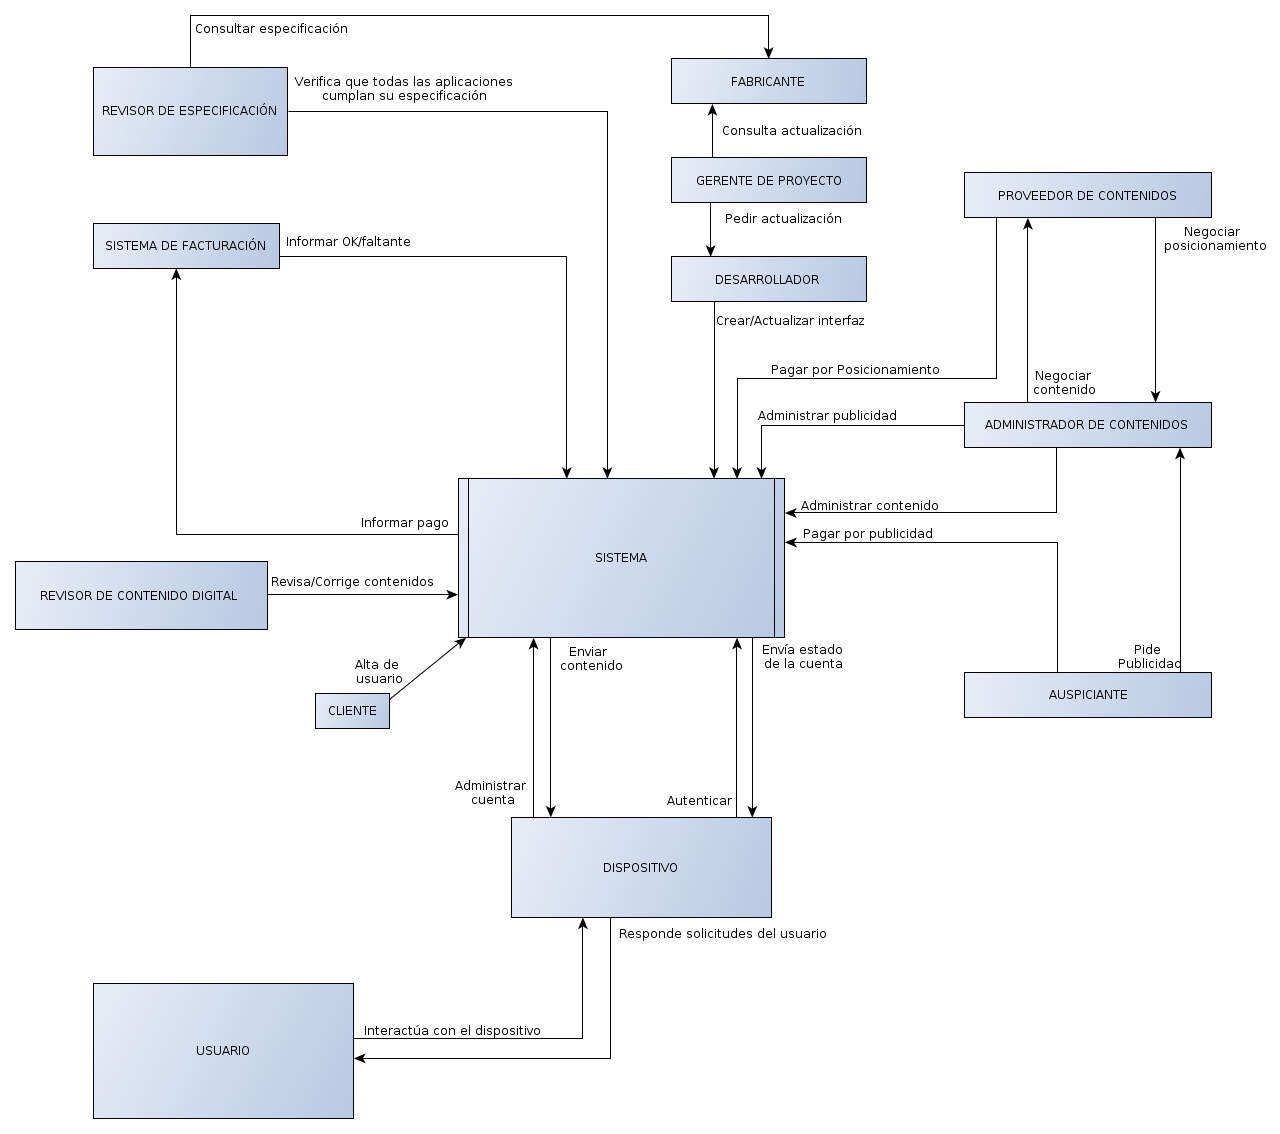
\includegraphics[scale=0.35]{Diagramas/DiagramaContexto.png}
	\end{center}

	El \emph{Sistema} se relaciona con varios agentes tanto directa como indirectamente. Ellos son:

	- Usuario: es la cuenta desde la cual el cliente se conectar\'a al sistema.
	El usuario interact\'ua con el sistema pudiendo autenticarse y Administrar su cuenta\\

		El cliente puede mediante la cuenta de usuario autenticarse para ser identificado en el sistema.
		Administrar el contenido engloba las siguientes acciones:

		\begin{itemize}
		\item{Comprar contenido}
		\item{Prestar contenido}
		\item{Pedir contenido}
		\end{itemize}

	
\section{Objetivos del sistema}

\subsection{Aclaraciones previas}

	A continuaci\'on describiremos el \emph{Modelo de Objetivos} que proponemos para cumplir los objetivos detallados anteriormente.

	El modelo se conforma por un arbol de objetivos y subobjetivos asociados, c\'omo dicho arbol es extremadamente grande se encuentra 
	dividido en varias partes. Por las reglas del modelo cada hoja del diagrama debe estar asociada a un \emph{agente}, en los casos en que
	una hoja no tenga un agente asociado tendr\'a un n\'umero que corresponde a otro gr\'afico donde el diagrama contin\'ua.
	
\subsection{Objetivos blandos}

\subsection{Modelo de Objetivos}

	\begin{center}
		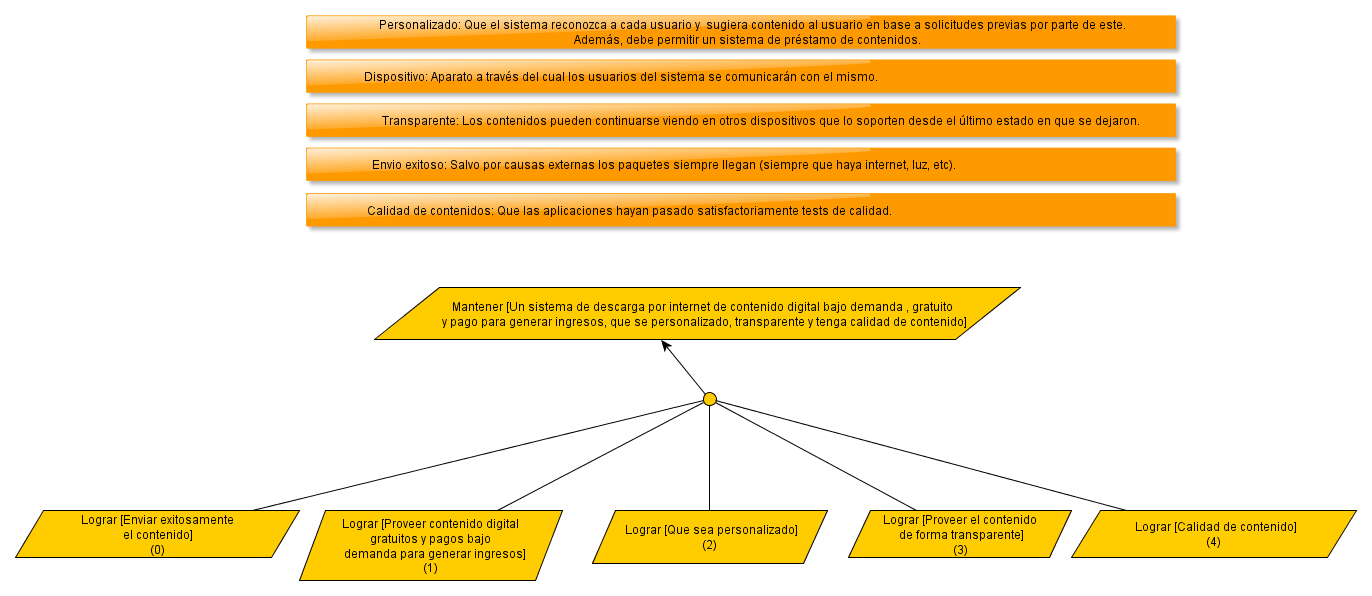
\includegraphics[scale=0.35]{Diagramas/ModelodeObjetivosPrincipal.png}
	\end{center}
	\begin{center}
		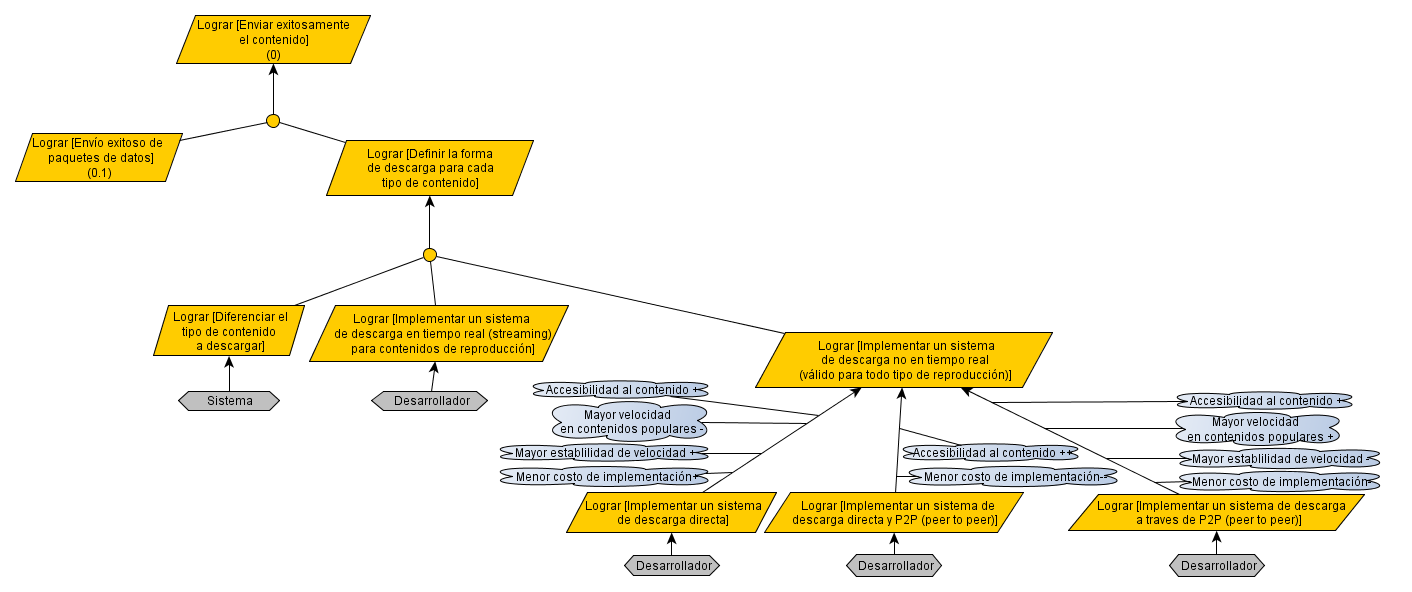
\includegraphics[scale=0.35]{Diagramas/0ModelodeObjetivosLograrenviarcontenido.png}
	\end{center}
	\begin{center}
		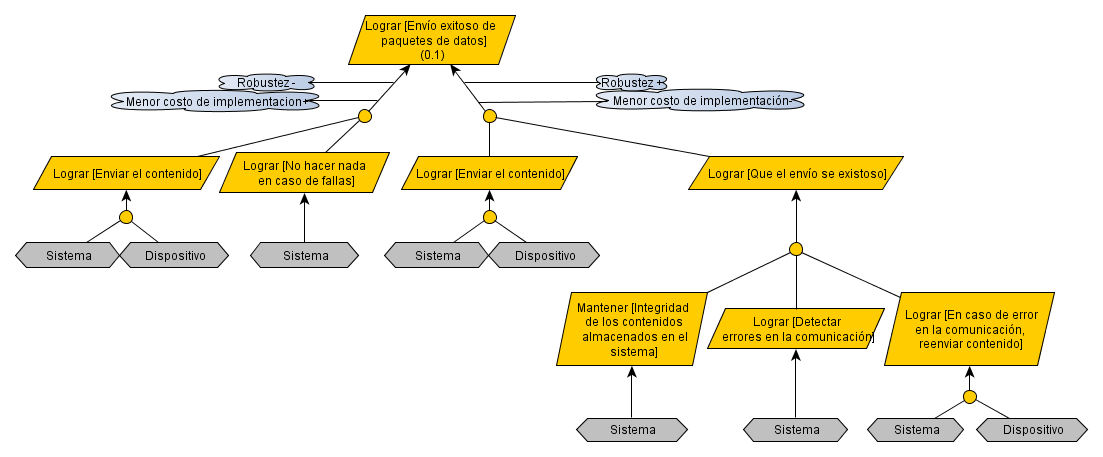
\includegraphics[scale=0.35]{Diagramas/0-1ModelodeObjetivosEnvioexitoso.png}
	\end{center}
	\begin{center}
		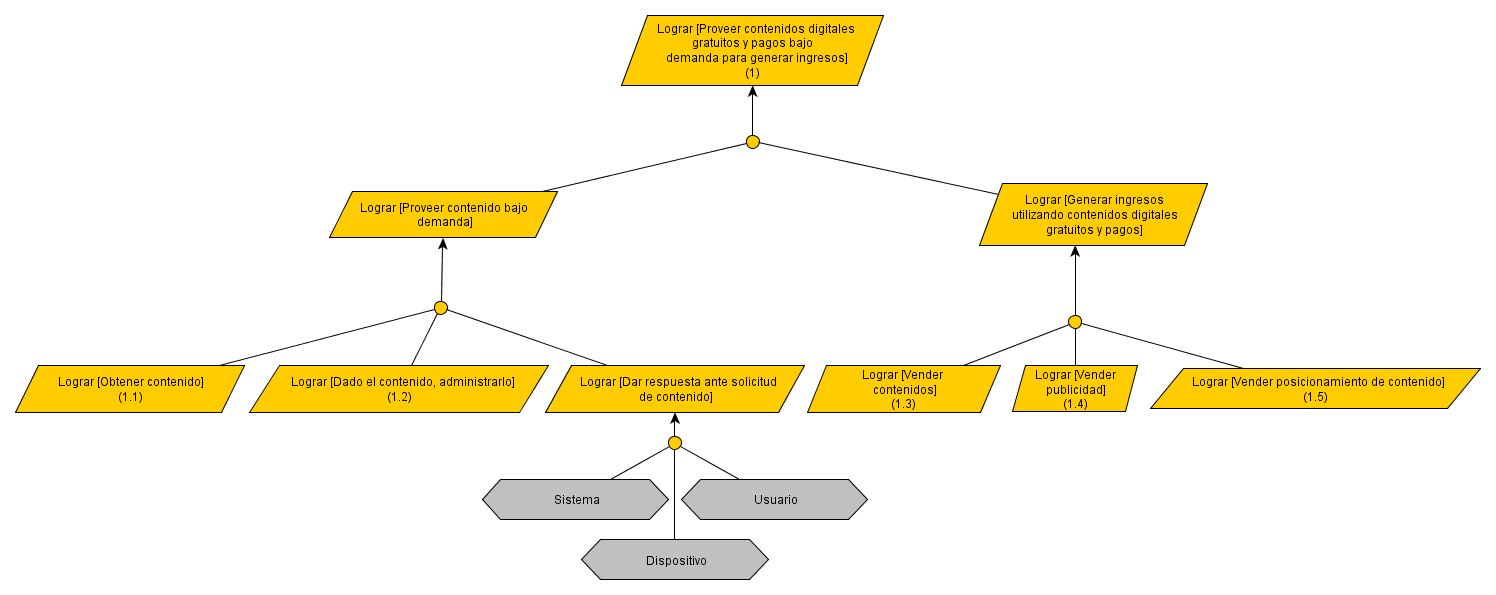
\includegraphics[scale=0.35]{Diagramas/1ModelodeObjetivosGenerarIngresos.png}
	\end{center}
	\begin{center}
		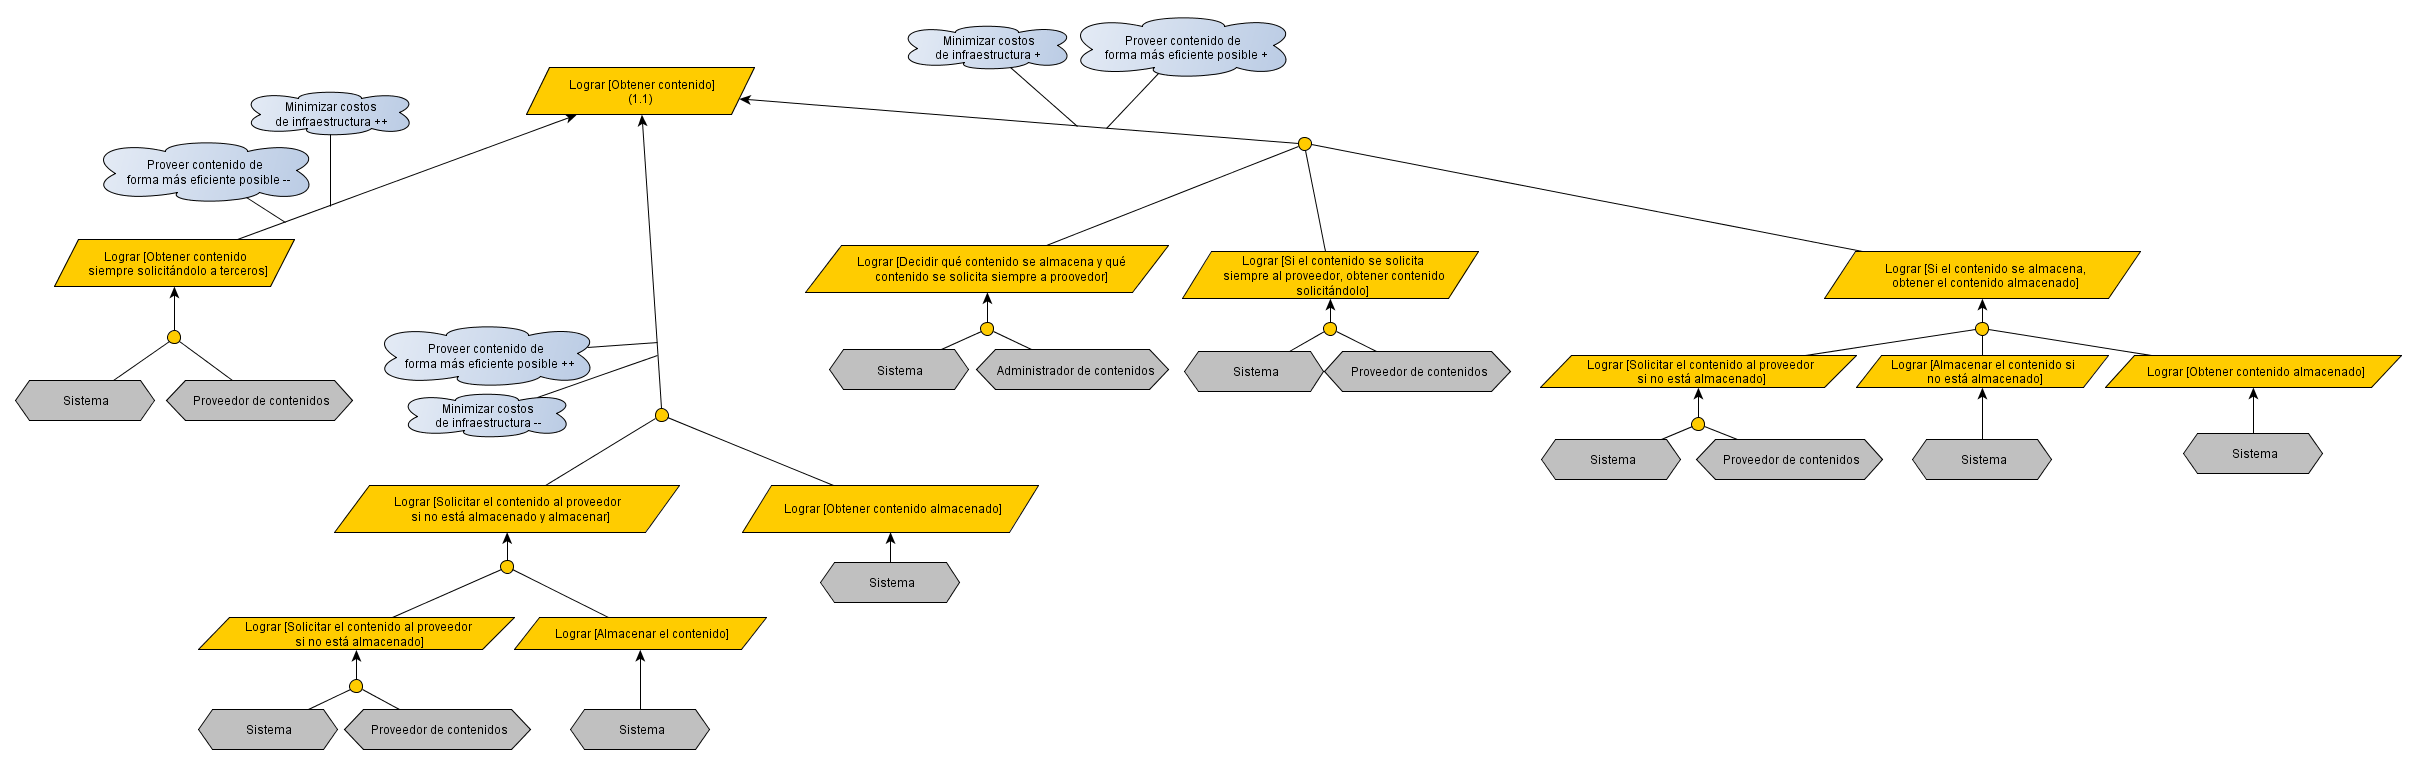
\includegraphics[scale=0.35]{Diagramas/1-1ModelodeObjetivosObtenercontenido.png}
	\end{center}
	\begin{center}
		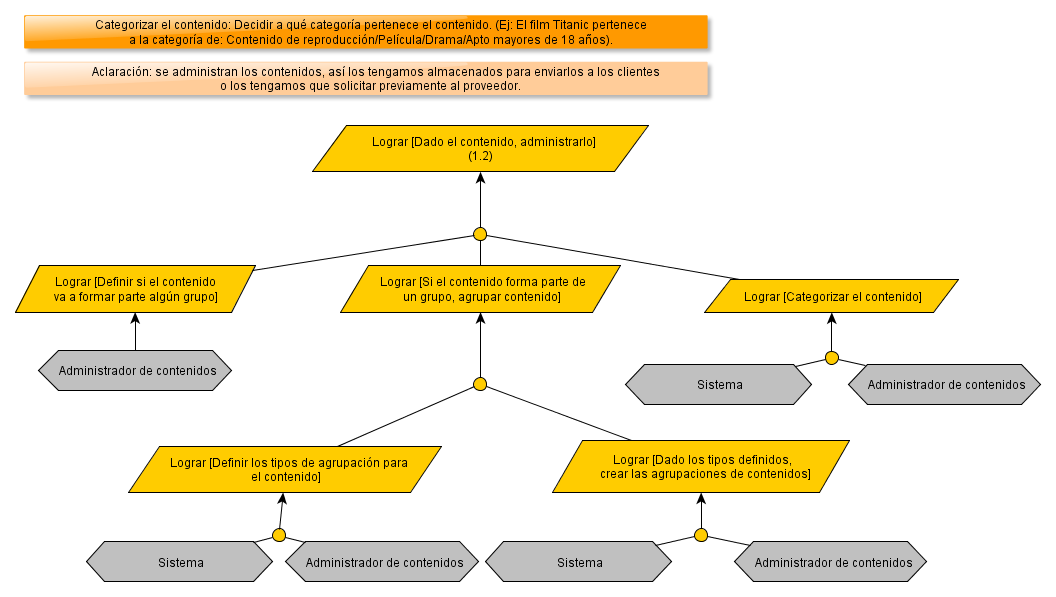
\includegraphics[scale=0.35]{Diagramas/1-2ModelodeObjetivosAdministrarcontenido.png}
	\end{center}
	\begin{center}
		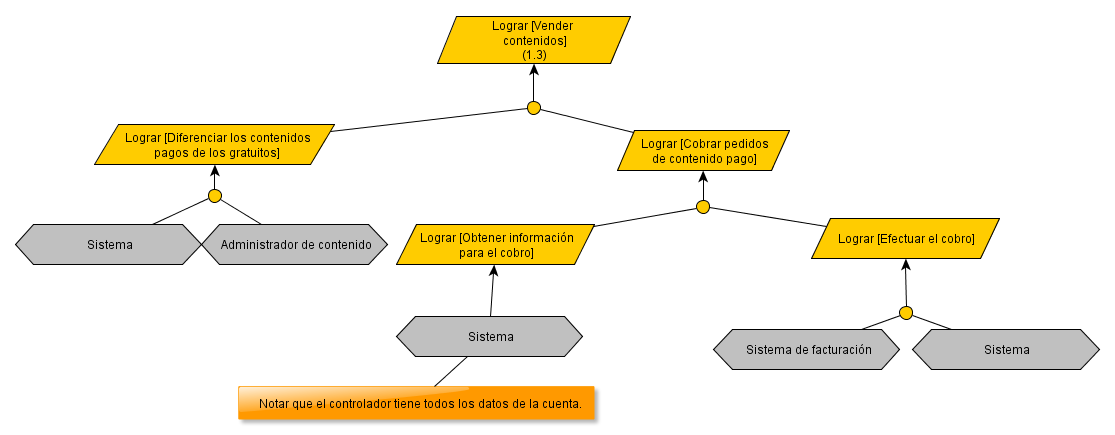
\includegraphics[scale=0.35]{Diagramas/1-3ModelodeObjetivosVendercontenido.png}
	\end{center}
	\begin{center}
		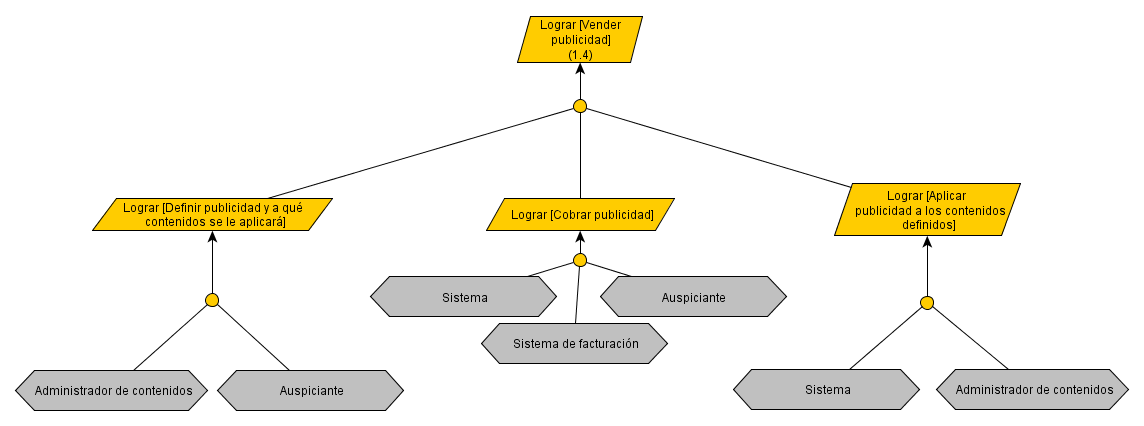
\includegraphics[scale=0.35]{Diagramas/1-4ModelodeObjetivosVenderpublicidad.png}
	\end{center}
	\begin{center}
		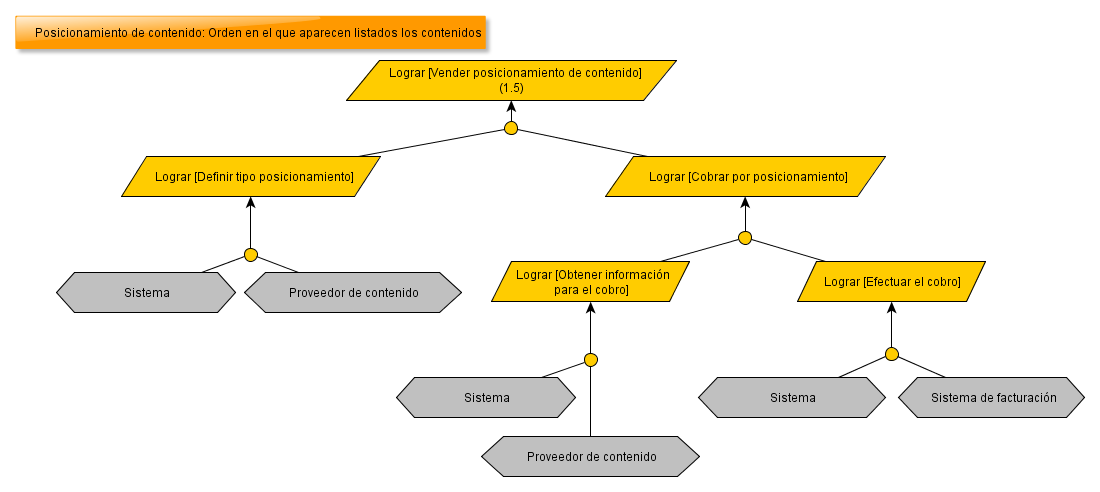
\includegraphics[scale=0.35]{Diagramas/1-5ModelodeObjetivosVenderposicionamiento.png}
	\end{center}
	\begin{center}
		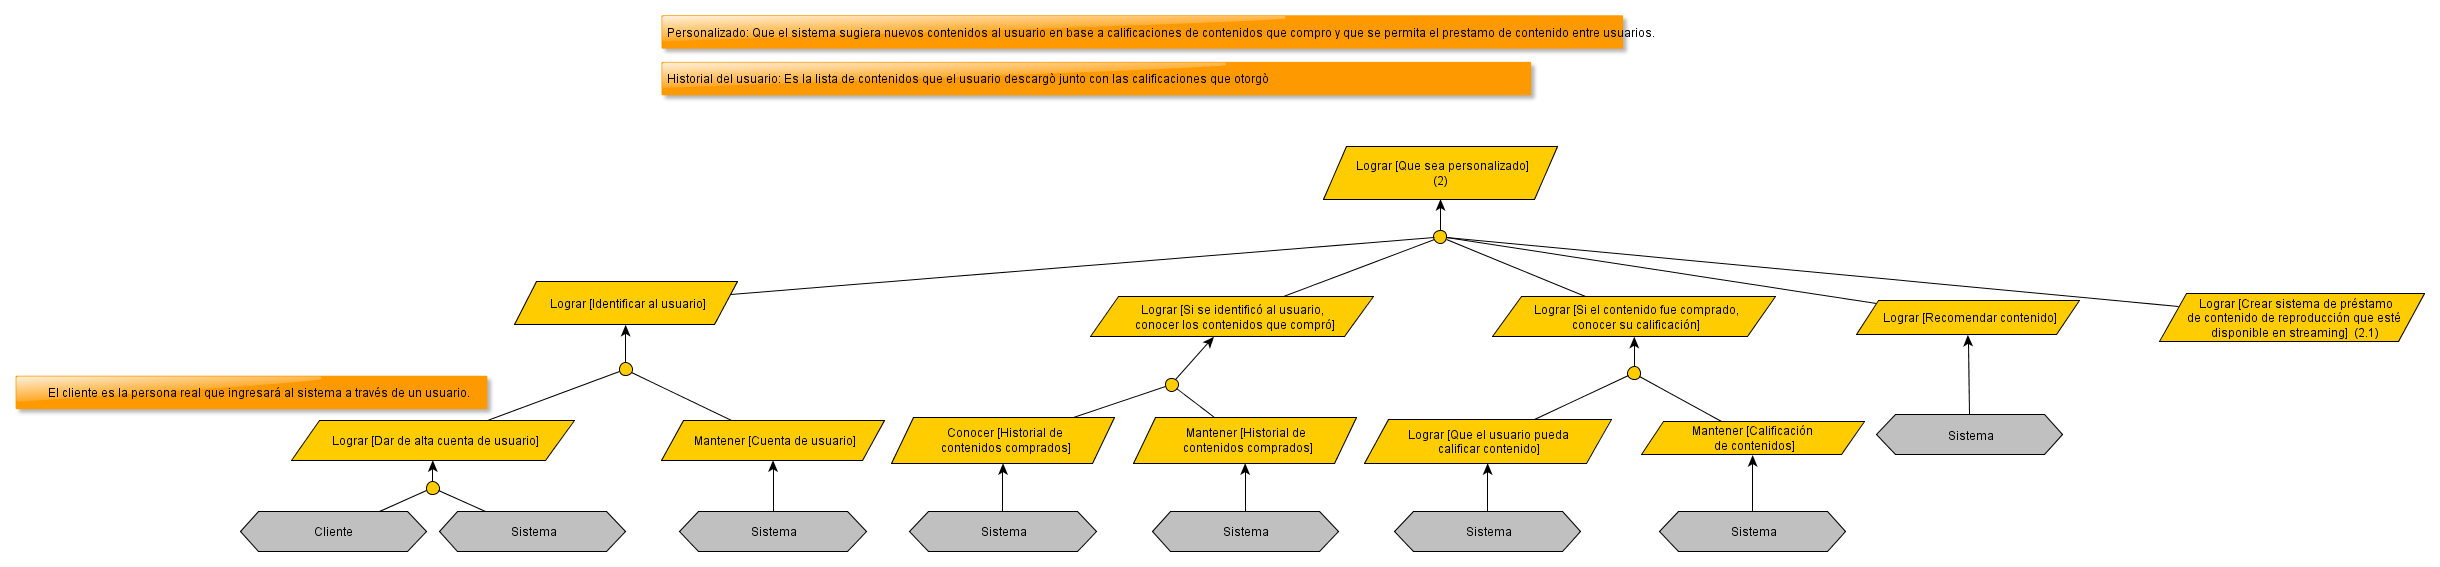
\includegraphics[scale=0.35]{Diagramas/2ModelodeObjetivosPersonalizado.png}
	\end{center}
	\begin{center}
		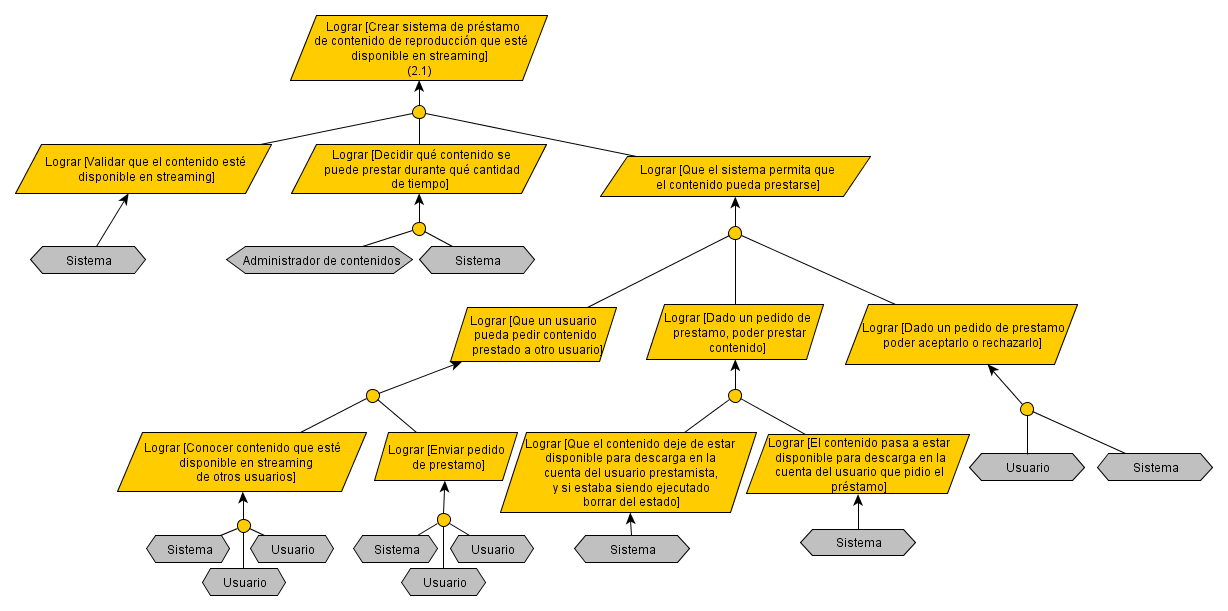
\includegraphics[scale=0.35]{Diagramas/2-1ModelodeObjetivosPrestamocontenidos.png}
	\end{center}
	\begin{center}
		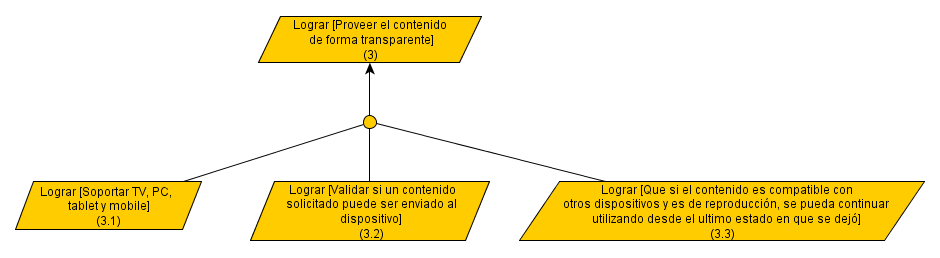
\includegraphics[scale=0.35]{Diagramas/3ModelodeObjetivosTransparente.png}
	\end{center}
	\begin{center}
		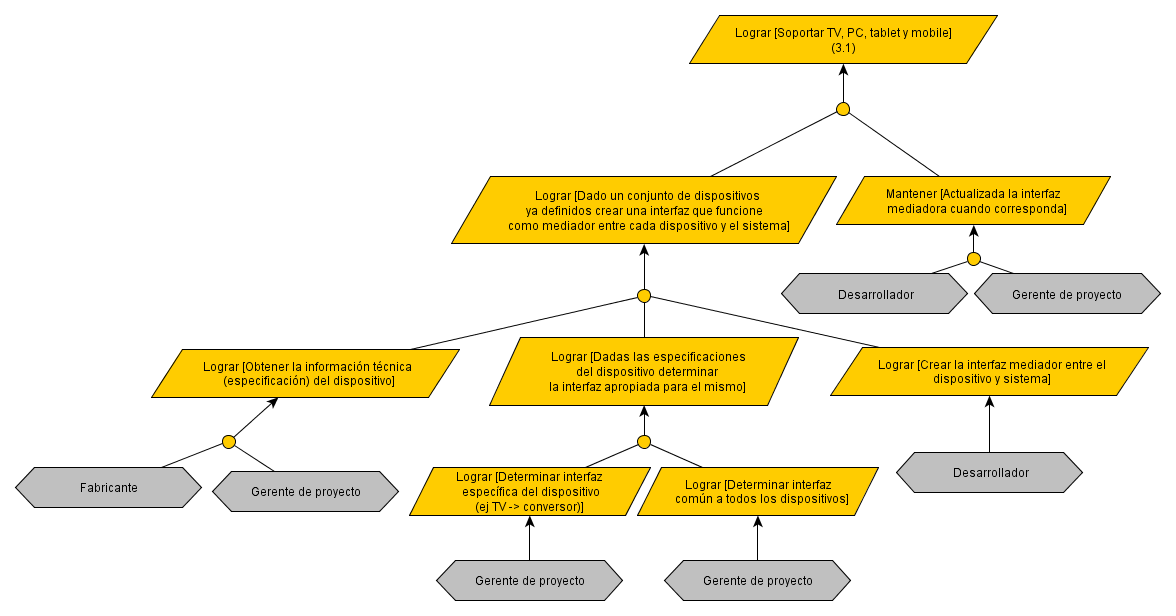
\includegraphics[scale=0.35]{Diagramas/3-1ModelodeObjetivosTransparencia.png}
	\end{center}
	\begin{center}
		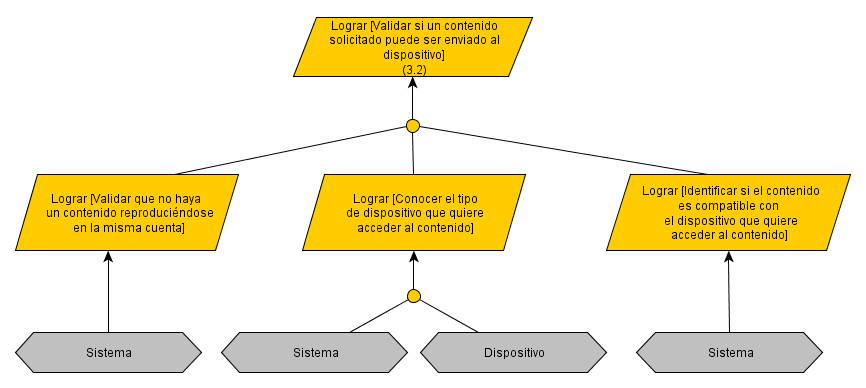
\includegraphics[scale=0.35]{Diagramas/3-2ModelodeObjetivosTransparencia.png}
	\end{center}
	\begin{center}
		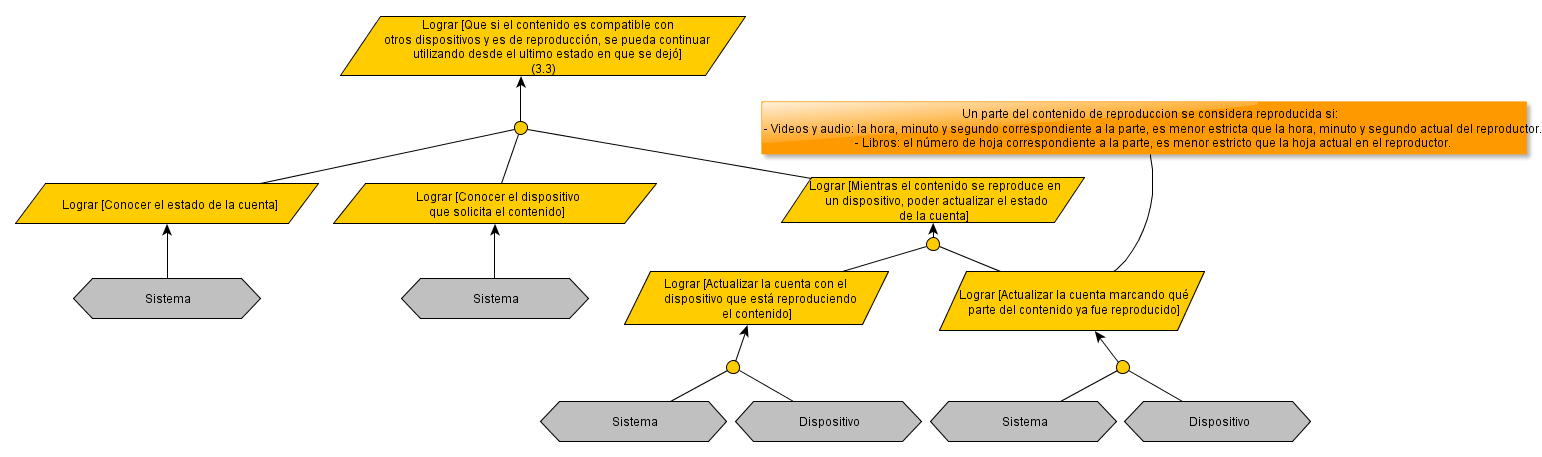
\includegraphics[scale=0.35]{Diagramas/3-3ModelodeObjetivosTransparencia.png}
	\end{center}
	\begin{center}
		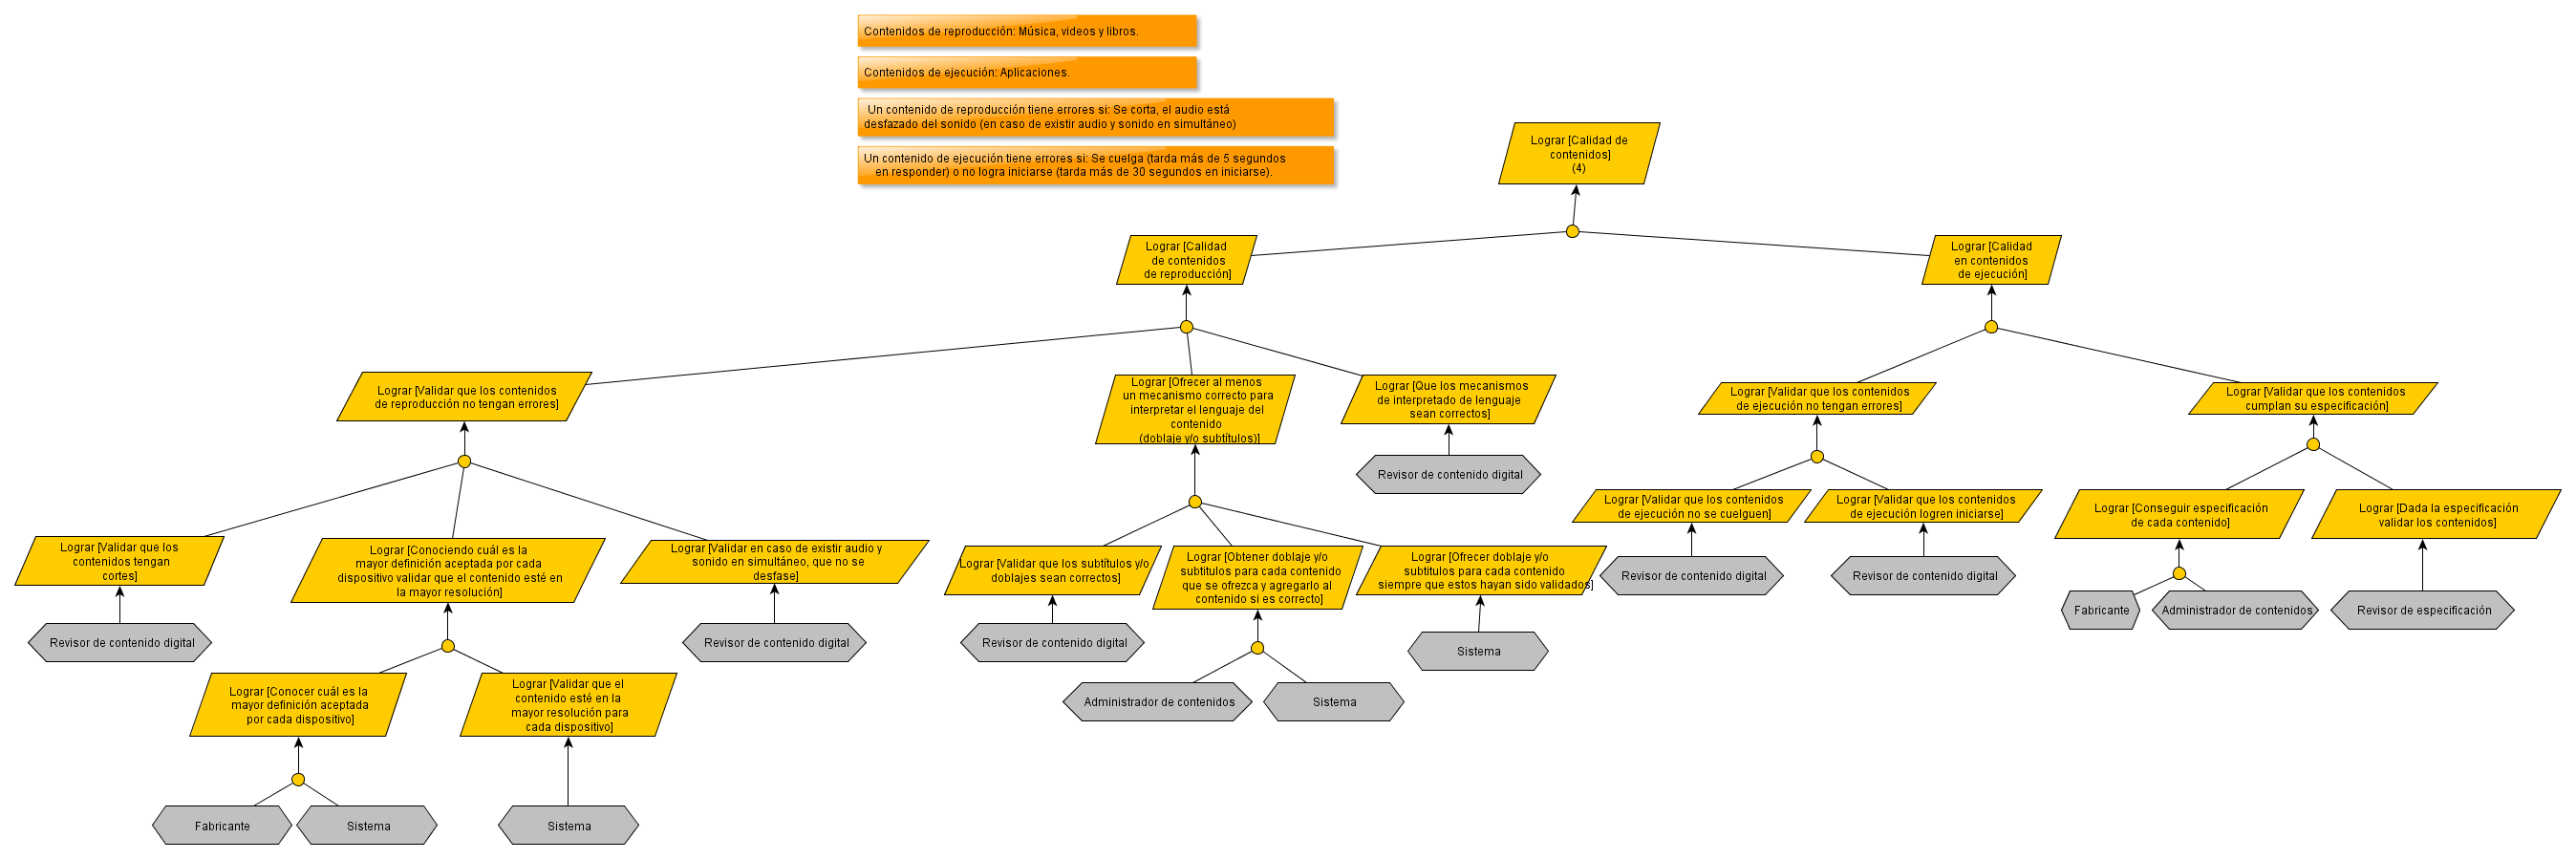
\includegraphics[scale=0.35]{Diagramas/4ModelodeObjetivosCalidaddecontenidos.png}
	\end{center}



\section{Asunciones}

	Dentro del sistema una cuenta de usuario no puede reproducir m\'as de un contenido por cuenta.
	Si se intenta reproducir otro contenido desde la misma cuenta el sistema no permitir\'a que se haga. 

	El sistema solo permite que los pr\'estamos de libros solo se otorguen por un m\'aximo de 8 semanas.

\newpage

\section{Escenarios informales y ejemplos}
	
	A continuaci\'on se describen una serie de casos que ejemplifican situaciones de funcionamiento esperado del sistema.

\subsection{Situaci\'on 1}

	\textbf{Funcionalidad:} Registro de usuario y baja de un contenido.\\

        Una persona se sienta en frente de la computadora.
    La persona se registra en el sistema (ingresa en la p\'agina del sitio, o descarga 
    la aplicaci\'on dependiendo de la implementaci\'on  de la interfaz de usuario).
    El controlador crea una cuenta y la asocia a esa persona (cliente). As\'i se crea el usuario.
    El usuario busca bajo la categor\'ia de deportes los partidos de f\'utbol locales.
    Encuentra el partido que buscaba (Chacarita vs Atlanta) y comienza a verlo desde su computadora (en streaming).\\

        En el entretiempo, se da cuenta que tiene que cocinar y no quiere dejar de ver el partido. Decide entonces loguearse al sistema desde su 
    tel\'efono inteligente (desde la p\'agina web del sitio o descargando la aplicaci\'on que corresponda). 
    Al autenticarse, la cuenta la cual posee el estado de reproducci\'on, le ofrece continuar viendo el partido desde el instante donde lo dej\'o.
    El cliente acepta y puede llegar a ver como Chacarita mete el segundo gol desde su cocina.

\subsection{Situaci\'on 2}

	\textbf{Funcionalidad:} Publicidad en contenidos.\\

        Un empresario de Powerthrist S.A. (bebida energ\'etica) desea publicitarse y se comunica con el administrador de contenidos de CentralMarket 
    envi\'andole el contenido a publicitar.
    El administrador de contenido le pasa el presupuesto junto con la lista de contenidos que pueden tener la publicidad.
    El empresario acepta y paga con v\'ia online (interactuando con el sistema) quien hace de intermediario con el sistema de facturaci\'on externo.
    El administrador de contenidos aplica entonces la publicidad sobre los contenidos acordados.
    Luego, los usuarios de CentralMarket que adquieran dichos contenidos se encuentran ahora con la publicidad de Powerthrist.

\subsection{Situaci\'on 3}

	\textbf{Funcionalidad:} Compra fallida y exitosa.\\

        Un usuario decide comprar la promoci\'on de verano de pel\'iculas de acci\'on (suponiendo que el gerente de CentralMarket ha dedicido agrupar el     
    contenido de esa forma). Efect\'ua el pago seleccionando de su cuenta una de sus tarjetas registradas. El sistema se comunica con el sistema de 
    facturaci\'on envi\'ando los datos del pago y recibe como respuesta que la tarjeta del usuario no tiene fondos. El sistema comunica al usuario el 
    resultado de la operaci\'on y se cancela la compra de la promoci\'on. El usuario recibe el mensaje y opta por elegir otra tarjeta y reintentar. Esta 
    vez la transacci\'on es exitosa y por consiguiente disfruta del contenido de la promoci\'on durante toda la temporada de verano.

\subsection{Situaci\'on 4}

	\textbf{Funcionalidad:} Obtenci\'on de contenidos y subt\'itulos y validaci\'on de los mismos.\\

        El administrador de contenidos conoce que ya se film\'o la nueva temporada de \emph{The Big Bang Theory}. Por lo tanto se comunica con el 
   proveedor de contenidos quien se los suministra. El administrador le pide adem\'as los subt\'itulos en espa�ol ya que la mayor\'ia de los subcriptores del 
   sistema son argentinos.

        Como debe cumplir los est\'andares de calidad de CentralMarket, una vez que el contenido ingresa al sistema este debe ser testeado por el revisor 
   de contenido digital previo a lanzamiento al p\'ublico. Es por ello que el revisor ve todos los cap\'itulos de la nueva temporada a publicar y valida 
   que ninguno de ellos se corte, adem\'as, tampoco nota ning\'un desfasaje entre la imagen y sonido. Nota que existen errores en el subt\'itulos por lo 
   tanto, el nuevo contenido todav\'ia no se puede proporcionar al p\'ublico.
   
      El administrador de contenidos vuelve a hablar con el proveedor, quien ahora le suministra unos nuevos subt\'itulos. Estos son vueltos a testear 
   con los cap\'itulos por el revisor quien finalmente los aprueba.

      De esta manera, la nueva temporada de la serie pasa a estar en el sistema como contenido a poder visualizarse. El administrador decide si va a    
   formar parte de un grupo, ser pago o gratuito y finalmente lo agrega al sistema.
   Los usuarios entonces pueden acceder a la reproducci\'on de la nueva serie aclamada de televisi\'on.

\subsection{Situaci\'on 5}

	\textbf{Funcionalidad:} Reproducci\'on de un mismo contenido de la misma cuenta desde dos dispositivos diferentes.\\

      Un usuario decide escuchar m\'usica v\'ia streaming desde su smartphone. El disco que decide escuchar es gratuito. Comienza a reproducirlo y su hija 
   se loguea al sistema con el mismo usuario desde su computadora de escritorio sin saber que su padre lo estaba utilizando desde su smartphone.\\

      La reproducci\'on no se inicia autom\'aticamente en la computadora y un mensaje aparece preguntando si se desea continuar desde el estado en que se   
   dej\'o (es decir en la canci\'on del disco que el padre est\'a escuchando actualmente). El padre no se entera que su hija se logue\'o.\\

      La hija decide no hacerlo, cancelando y entrando a la lista de contenidos de CentralMarket. Encuentra una serie para ver y clickea sobre ella. Se 
   levanta un cartel que dice ``Actualmente hay un contenido en reproducci\'on/descarga. La operaci\'on que ud. desea hacer no puede ser realizada.`` 	  y se vuelve al listado de contenidos.

\subsection{Situaci\'on 6}

	\textbf{Funcionalidad:} Actualizaci\'on de la interfaz del usuario.\\

	Supongamos que la interfaz de CentralMarket consiste en una aplicaci\'on que se instala en los dispositivos.

	Se confirma que se va a sacar un nuevo Service Pack para el sistema operativo Windows 7. Este Service Pack realiza una modificaci\'on sobre la   
   API de Windows lo que provocar\'ia que todos los usuarios utilizando CentralMarket desde una computadora con Windows 7 no puedan utilizar el servicio 
   de forma correcta.\\

       El gerente de proyecto est\'a al tanto de la situaci\'on, se comunica entonces con el fabricante, en este caso la gente de Microsoft y pide el    
   detalle sobre la nueva interfaz de comunicaci\'on con el SO (detalle de la API modificada). Con esta informaci\'on se encarga de avisarle al 
   desarrollador para poder sacar una nueva versi\'on del sistema de CentralMarket compatible con el release del Service Pack de Windows.

\subsection{Situaci\'on 7}

	\textbf{Funcionalidad:} Pr\'estamo de un libro.\\

	Miguel, un cliente de CentralMarket se entera que su amigo Carlos tambi\'en es cliente de la misma compa�\'ia. Decide buscar mediante el sistema    
   qu\'e contenido posee Carlos en su cuenta y encuentra que hace m\'as de un a�o compr\'o ``Vuelta al mundo en 80 d\'ias`` de Julio Verne, el libro que siempre quiso leer pero nunca tuvo oportunidad. Decide ped\'irselo prestado por 8 semanas, lapso que el sistema establece para el pr\'estamo de dicho contenido. \\

        En ese momento, Carlos se encontraba reley\'endolo, pero decide prest\'arselo de todas formas. Unas semanas m\'as tarde, Carlos accede a  CentralMarket con el objeto de continuar leyendo su libro. Una vez que accede, se da cuenta que el libro sigue prestado y debe por lo tanto, esperar a que Carlos se lo devuelva teniendo como l\'imite el plazo fijado por el sistema. 

\subsection{Situaci\'on 8}

	\textbf{Funcionalidad:} Autenticaci\'on err\'onea.\\

	Un cliente de CentralMarket desea loguearse al sistema para descargar juegos. Entra al sitio (o abre la aplicaci\'on, dependiendo de la interfaz 
   utilizada), ingresa su nombre de usuario y pone su contrase�a. La contrase�a es incorrecta por lo que el sistema le avisa y lo invita a reintentar. 
   Nuevamente la ingresa incorrectamente y nuevamente es avisado.
   Este procedimiento puede realizado infinitas veces.

\subsection{Situaci\'on 9}

	\textbf{Funcionalidad:} Posicionamiento de contenido.\\

	Uno de los proveedores de contenido de CentralMarket desea publicitar una de sus series , una sitcom llamada ``�� Qui\'en me mand\'o a estudiar    
   computaci\'on?!``, que debido a su poco \'exito no est\'a consiguiendo cubrir los costos de su producci\'on, y para esto se comunica con el administrador de 
   contenido quien le informa que si paga la tarifa adecuada, este puede posicionarla en los primeros lugares cuando los usuarios realicen alguna    
   b\'usqueda en la cual esta sitcom est\'e relacionada. Al aceptar, el proveedor de contenido realiza el pago en el sistema, y espera que las cr\'iticas    
   mejoren para poder vender una nueva temporada de su serie a las cadenas televisivas y otras empresas. 


\subsection{Situaci\'on 10}

	\textbf{Funcionalidad: } .\\

	Un usuario decide poder acceder a un contenido. Por lo tanto se loguea al sistema, lo busca entre la lista de contenido y lo selecciona, para 
   accederlo. Desde el sistema, se recibe el pedido y lo procesa.\\

       Si se trata de un contenido gratuito, lo obtiene. Si se trata de un contenido pago, el sistema coteja el producto solicitado con el historial de compras del usuario para determinar si debe cobrarle el acceso o no. En caso de que ya lo haya comprado, obtiene el contenido; sino le ofrece la opci\'on de compra.\\
       La forma de obtenerlo depender\'a del refinamiento elegido. Puede ser alguna de las siguientes:

	\begin{itemize}
	
	\item{ El sistema se comunica con la interfaz del proveedor que posee ese contenido, requiri\'endoselo. El contenido le llega al sistema que lo re-codifica para ser entendible por el dispositivo del usuario. Dependiendo del tr\'afico de red o carga de procesamiento del proveedor, el sistema, y por consiguiente el usuario, puede llegar a quedarse esperando indefinidamente respuesta.}

	\item{ El sistema recibe el pedido y debe requerirselo al proveedor si el contenido no est\'a en el sistema, almacen\'andolo a medida que realiza el env\'io al usuario para en posteriores pedidos, ya tenerlo disponible y no necesitar pedirlo al proveedor. Si est\'a almacenado, simplemente comienza la transferencia.}

	\item{e Para minimizar los costos de mantenimiento de infraestructura, el administrador de contenidos decide que (dada la posibilidad que ofrece el sistema de elegir cu\'ando guardar el contenido en servidores propios) se van a almacenar s\'olo los contenidos que se hayan solicitado m\'as de 100 veces en el lapso de una semana, quiere as\'i minimizar el tr\'afico de red y economizar espacio.}

	De Lunes a S\'abado recibe 99 pedidos de descarga de un juego de videos para la computadora. En cada uno de estos pedidos, el sistema se comunica con el proveedor pidi\'endole el contenido y d\'andoselo al usuario.

	El d\'ia domingo recibe el pedido n\'umero 100 y por lo tanto debe esta vez pedirlo al proveedor y a su vez almacenarlo. Resulta ser una buena desici\'on ya que en el correr de la semana siguiente, se realizan cientos de pedidos del mismo juego a CentralMarket y se logra evitar el tr\'afico de red con el proveedor.

	\end{itemize}

\end{document}
